\documentclass[]{article}
\usepackage{graphicx}
\usepackage[]{amsmath}

\title{Relatório do Trabalho Final de Circuito Digital}
\author{Erickson Müller, mat: 20230001178\\ Erickson Müller, mat: 20230001178}
\date{04 de julho de 2024}

\begin{document}
\maketitle
\pagebreak
\section{Introdução}
	O objetivo desse trabalho é apresentar os resultados da implementação do circuito lógico apresentado pelos professores Geomar André Schreiner e Luciano Lores Caimi, conforme imagem abaixo:
	\\
	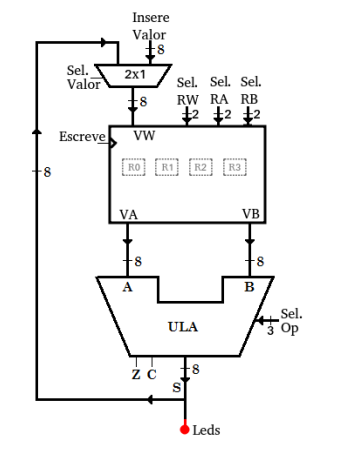
\includegraphics[scale=0.8]{Images/Circuito Lógico.png}
	\\
	O projeto foi montado no programa Logisim-Evolution v3.8.0, usando os componentes do \textit{software}. Ao total, foram montados 10 subcircuitos, acrescidos do circuito \textit{main}; O circuito possui 5 chaves seletoras (estas representando em ordem binária as entradas/saídas de cima para baixa), 1 entrada de 8 bits para inserir valor, e duas entradas que funcionam como enable e clock dos flip-flops. Com esse circuito, podemos resolver equações de segundo grau e binômios quadrados.
	
	
	
	\newpage
\section{Descrição da Solução}
	
	\subsection{Diagrama com os Blocos Operacionais}
		O projeto possui ao todo 10 subcircuitos que interagem entre sim são utilizados para o sucesso do circuito principal. A seguir apresentamos imagens destas estruturas:
		\begin{enumerate}
		
		\item Circuito Principal\\
		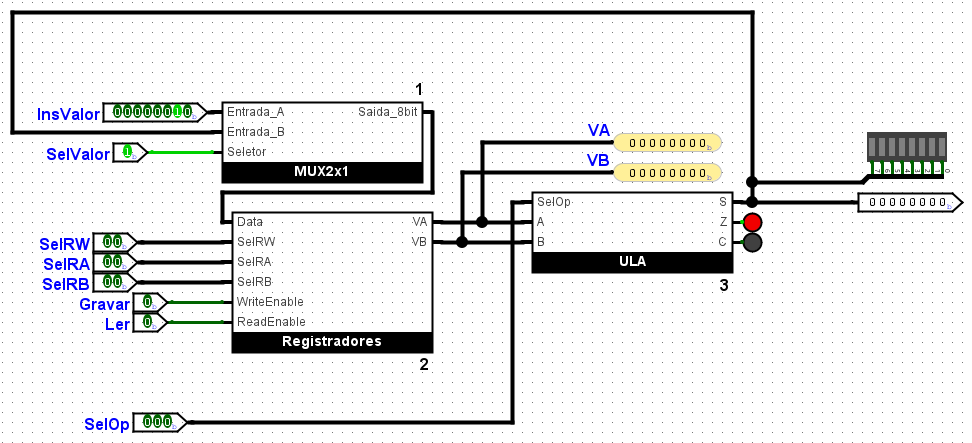
\includegraphics[scale=0.5]{Images/main.png}\\
		\item Banco de Registradores\\
		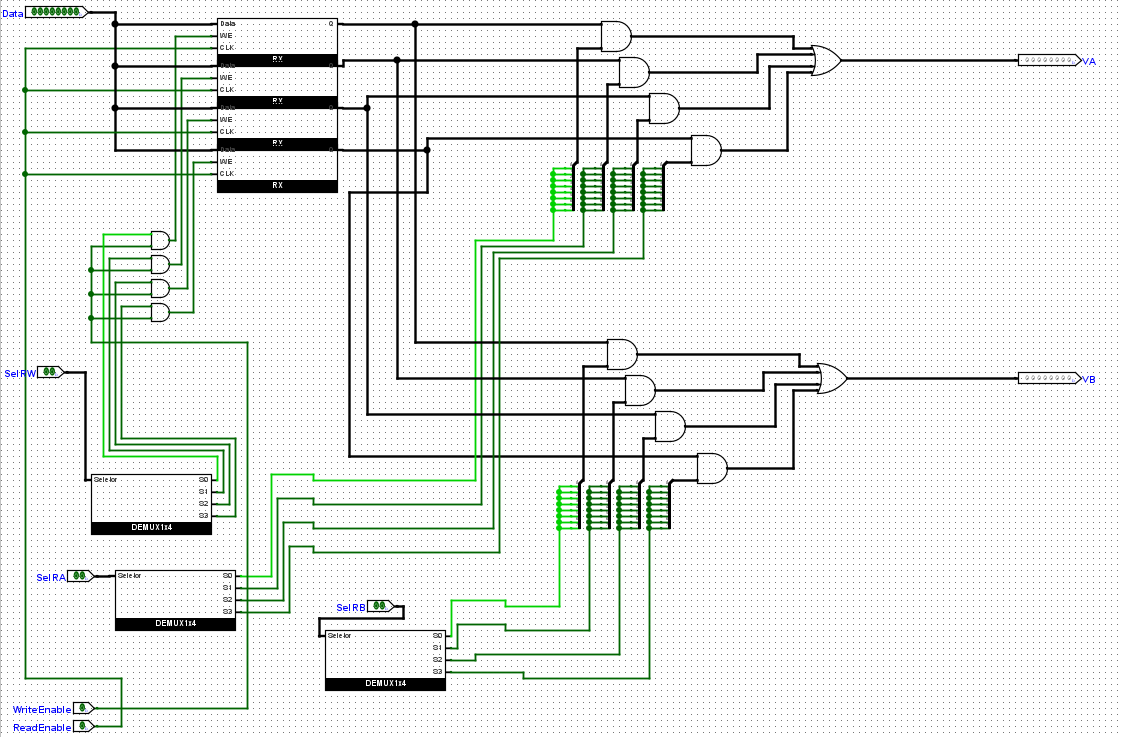
\includegraphics[scale=0.4]{Images/Registradores.png}\\
		\newpage
		\item Registrador de 8 bits montado com flip-flops\\
		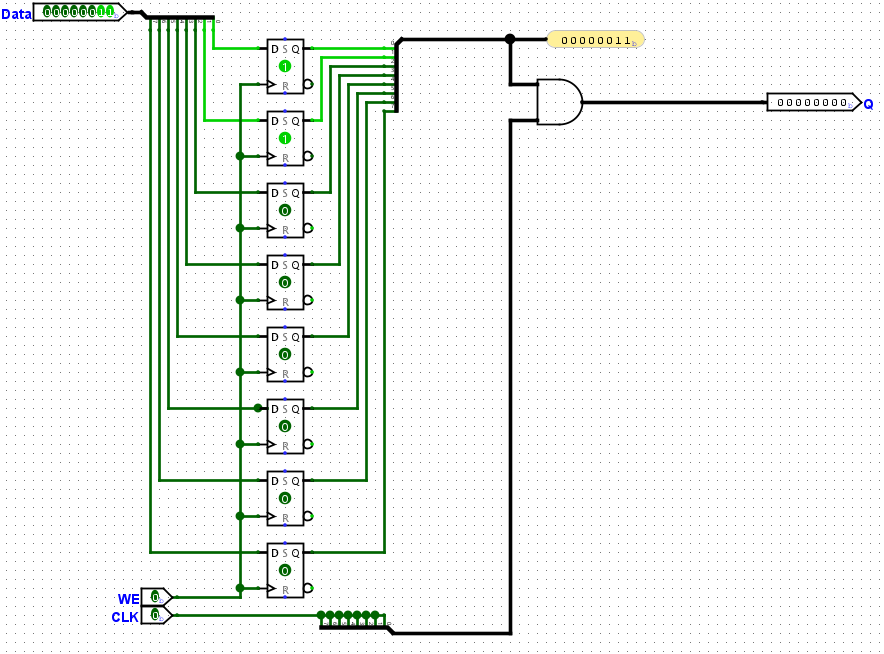
\includegraphics[scale=0.5]{Images/RX.png}\\
		\item Unidade Lógica Aritmética (Dupla 31)\\
		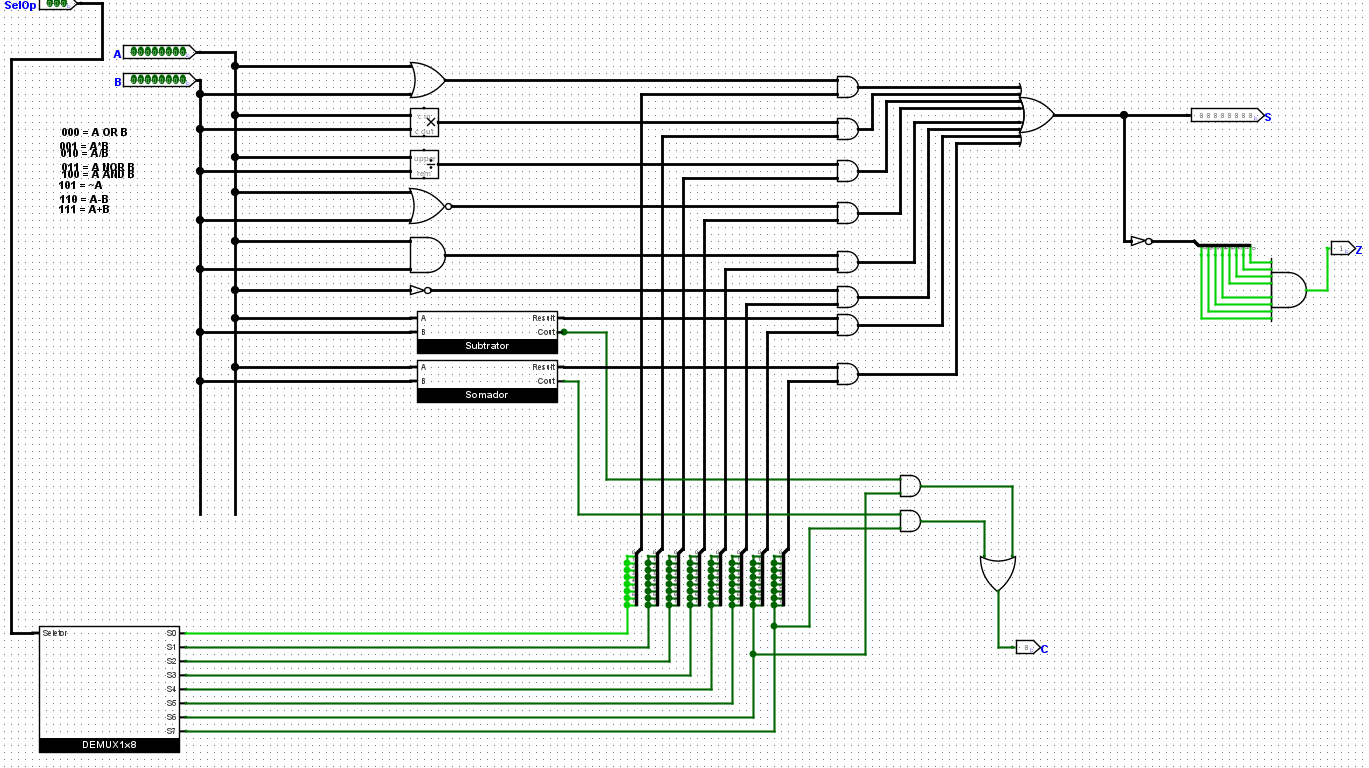
\includegraphics[scale=0.4]{Images/ULA.png}\\
		\item Somador de 1 bit, utilizado nos subcircuitos de somador e subrator\\
		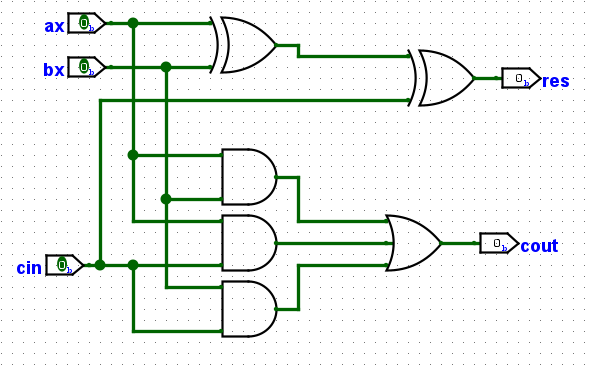
\includegraphics[scale=0.8]{Images/Somador1bit.png}\\
		\item Somador de 8 bits\\
		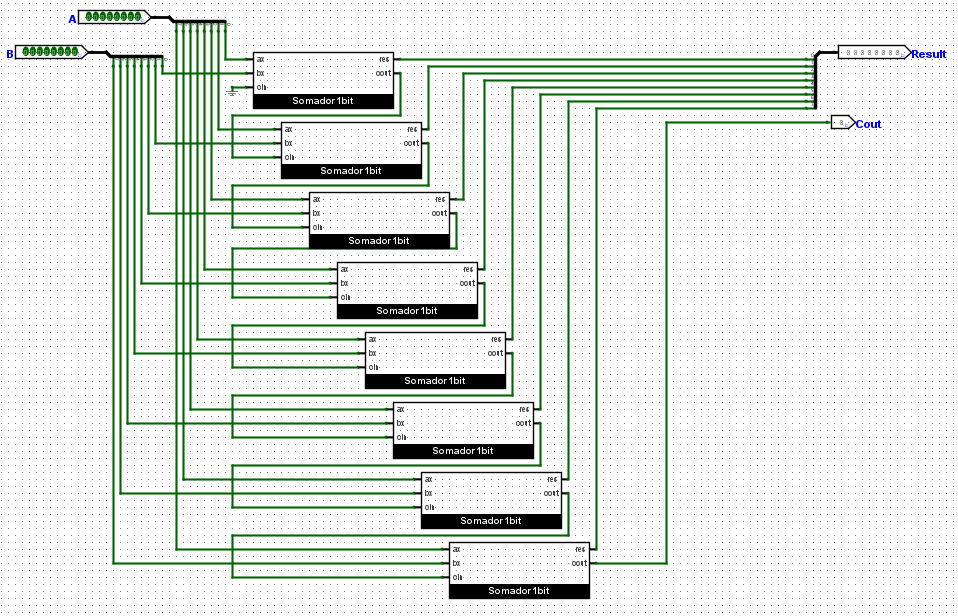
\includegraphics[scale=0.55]{Images/Somador.png}\\
		\item Subtrator de 8 bits\\
		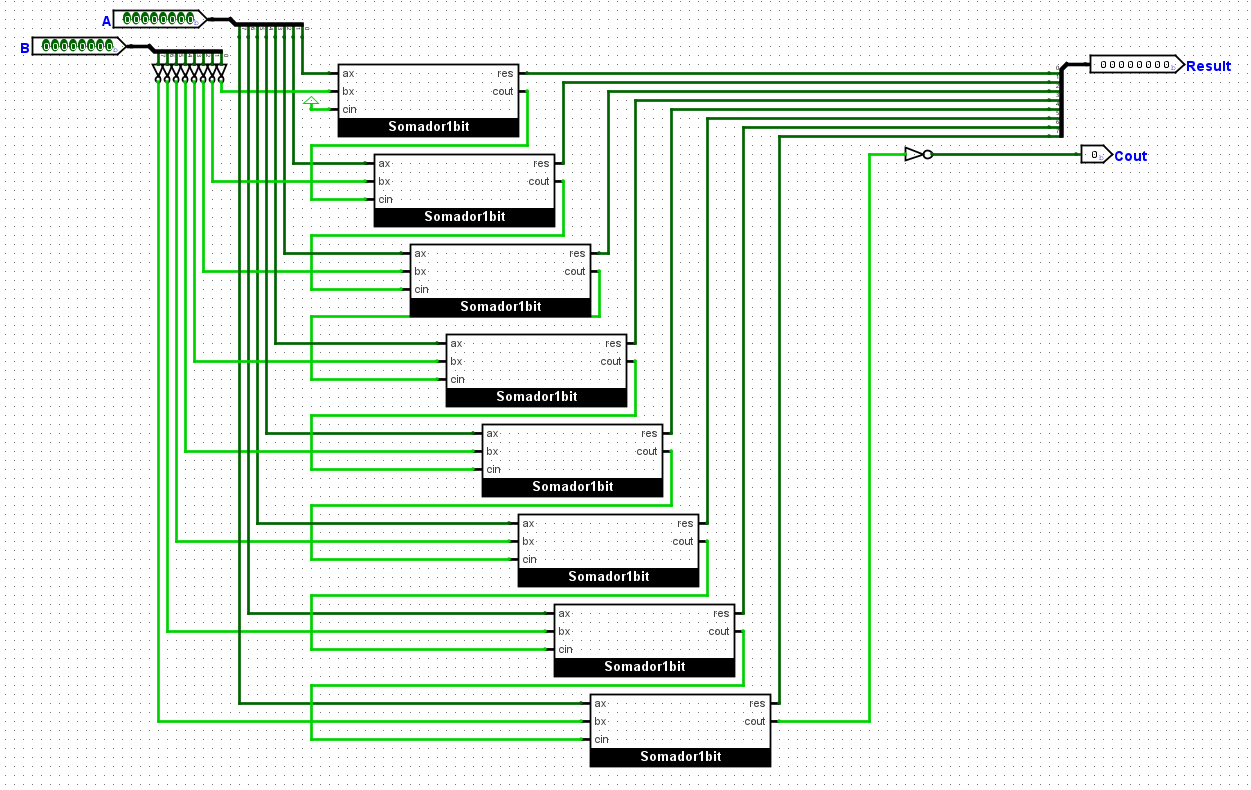
\includegraphics[scale=0.45]{Images/Subtrator.png}\\
		\newpage
		\item Multiplexador 2x1\\
		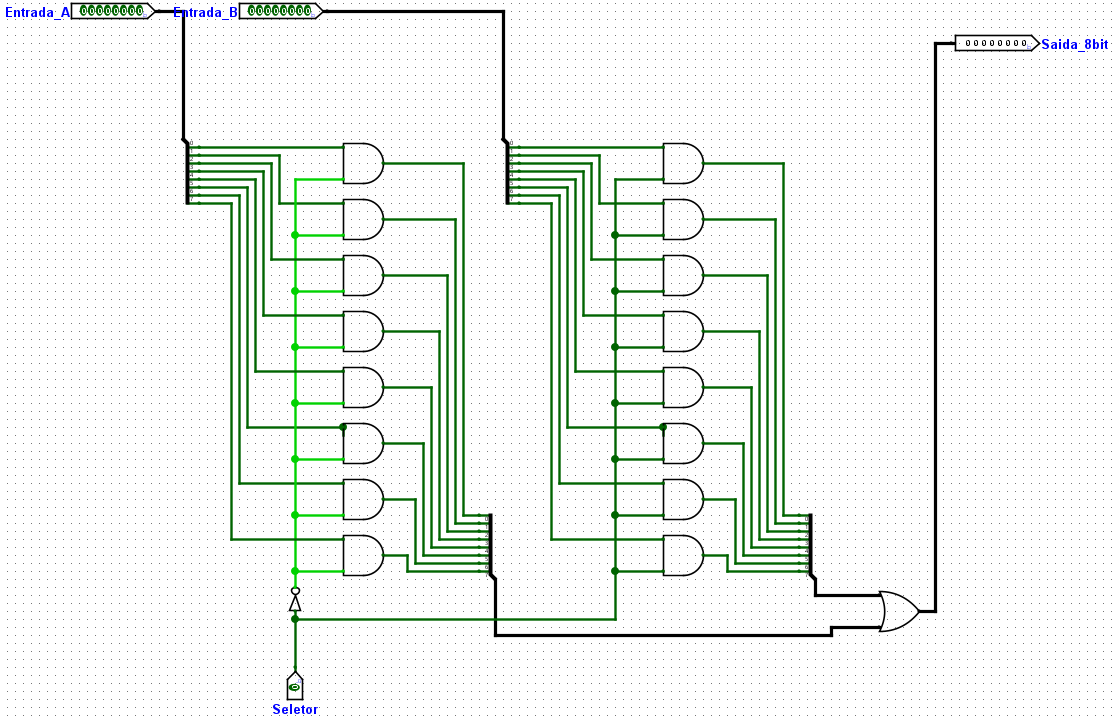
\includegraphics[scale=0.5]{Images/MUX2x1.png}\\
		\item Multiplexador 4x1\\
		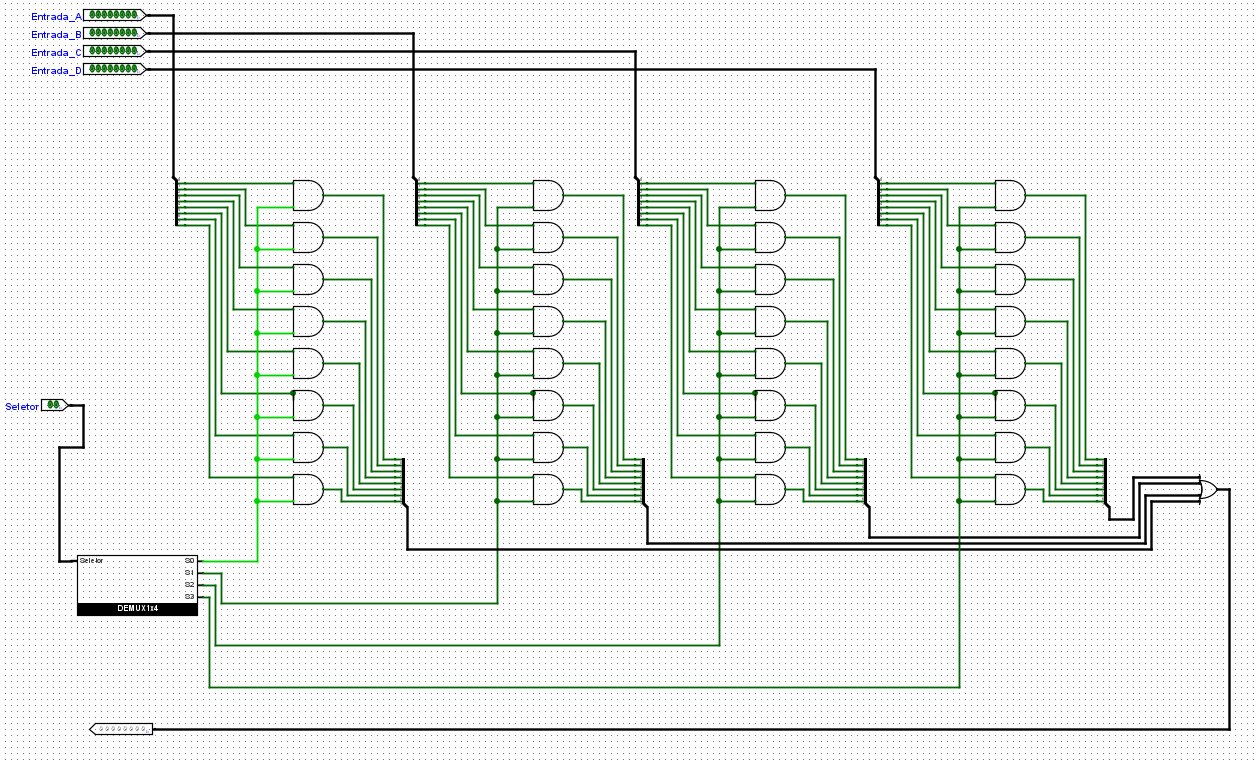
\includegraphics[scale=0.4]{Images/MUX4x1.png}\\
		\item Demultiplexador 1x4\\
		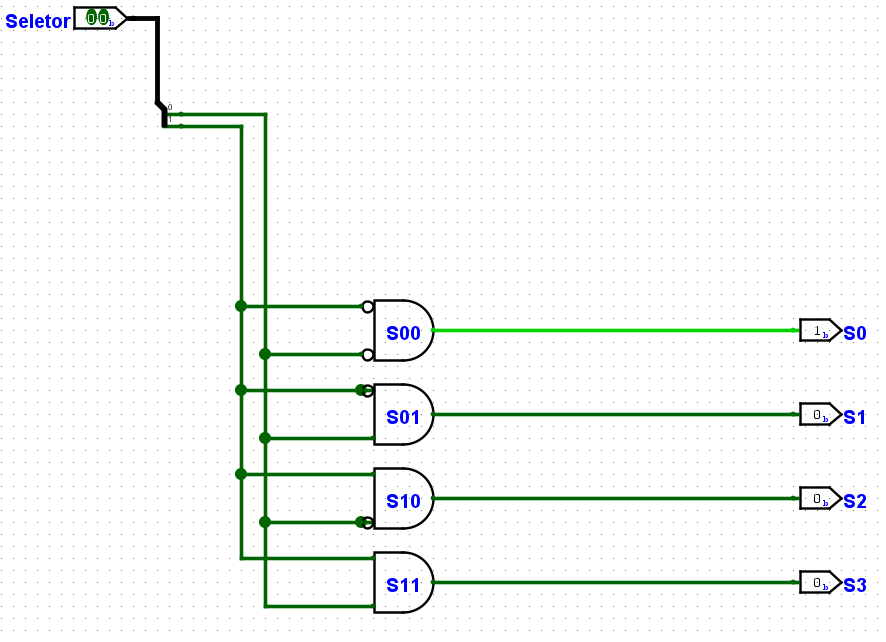
\includegraphics[scale=0.5]{Images/DEMUX1x4.png}\\
		\item Demultiplexador 1x8\\
		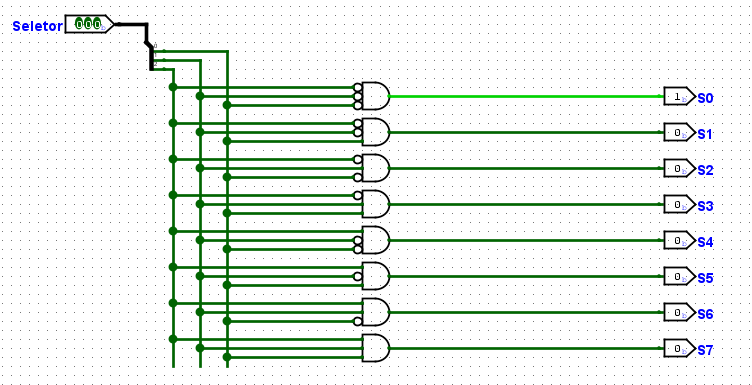
\includegraphics[scale=0.6]{Images/DEMUX1x8.png}\\

		\end{enumerate}
	\subsection{Equações propostas}
		A nossa dupla optou pela ordem de seleção da ULA do Grupo 31, conforme imagem abaixo. Essas operações vão ser utilizadas na resolução da função quadrática e do binômio quadrado.\\
		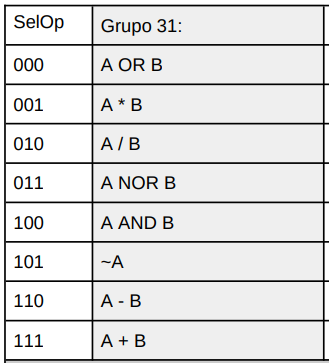
\includegraphics[scale=0.9]{Images/SelOp.png}\\
		
		A função quadrática a ser solucionada é a seguinte: $$y = 2x^2+3x-4$$
		Para os valores de $x$, foram atribuidos os números $2$ e $-2$\\
		\\
		O binômio quadrado a ser solucionado é o seguinte: $$(3+5)^2 = 3^2 +2.3.5 +5^2$$
		Iremos armazenar os valores de cada lado da equação em um registrador e subtrair, resultando no valor 0, que acenderá o led $Z$.
		
	\subsection{Soluções da Função de Segundo Grau com x = 2}
		Após zerar todas as entradas:
		\begin{enumerate}
			\item InsValor = 00000010 (Armazenar 2 no R0)
			\\ SelRW = 00
			\\ Gravar = 1,0
			
			\item InsValor = 00000011 (Armazenar 3 no R1)
			\\ SelRW = 01
			\\ Gravar = 1,0
			
			\item InsValor = 11111100 (Armazenar -4 no R2)
			\\ SelRW = 10
			\\ Gravar = 1,0
			
			\item InsValor = 00000010 (Armazenar 2 no R3)
			\\ SelRW = 11
			\\ Gravar = 1,0
			
			\item SelRA = 01 (Multiplicar B e X)
			\\ SelRB = 11
			\\ SelOp = 001
			\\ Ler = 1
			
			\item SelValor = 1 (Armazenar b.x no R1)
			\\ SelRW = 01
			\\ Gravar = 1
			\\ Ler = 0
			\\ Gravar = 0
			
			\item SelRA = 11 (Multiplicar X e X)
			\\ Sel RB = 11
			\\ Ler = 1
			
			\item SelRW = 11 (Armazenar $x^2$ no R3)
			\\ Gravar = 1
			\\ Ler = 0
			\\ Gravar = 0
			
			\item SelRA = 00 (Multiplicar A e $x^2$)
			\\ SelRB = 11
			\\ Ler = 1
			
			\item SelRW = 00 (Armazenar $a.x^2$ no R0)
			\\ Gravar = 1
			\\ Ler = 0 
			\\ Gravar = 0
			
			\item SelRA = 00 (Somar $a.x^2 + b.x$)
			\\ SelRB = 01
			\\ SelOp = 111
			\\ Ler = 1
			
			\item SelRW = 00 (Armazenar $a.x^2 + b.x$ no R0)
			\\ Gravar = 1
			\\ Ler = 0
			\\ Gravar = 0 
			
			\item SelRA = 00 (Somar $a.x^2 + b.x$ e c)
			\\ SelRB = 10
			\\ Ler = 1
			
		\end{enumerate}
		Resultado = 10.
		
	\subsection{Soluções da Função de Segundo Grau com x = -2}
		Após zerar todas as entradas:
		\begin{enumerate}
			\item InsValor = 00000010 (Armazenar 2 no R0)
			\\ SelRW = 00
			\\ Gravar = 1,0
			
			\item InsValor = 00000011 (Armazenar 3 no R1)
			\\ SelRW = 01
			\\ Gravar = 1,0
			
			\item InsValor = 11111100 (Armazenar -4 no R2)
			\\ SelRW = 10
			\\ Gravar = 1,0
			
			\item InsValor = 11111110 (Armazenar -2 no R3)
			\\ SelRW = 11
			\\ Gravar = 1,0
			
			\item SelRA = 01 (Multiplicar B e X)
			\\ SelRB = 11
			\\ SelOp = 001
			\\ Ler = 1
			
			\item SelValor = 1 (Armazenar b.x no R1)
			\\ SelRW = 01
			\\ Gravar = 1
			\\ Ler = 0
			\\ Gravar = 0
			
			\item SelRA = 11 (Multiplicar X e X)
			\\ Sel RB = 11
			\\ Ler = 1
			
			\item SelRW = 11 (Armazenar $x^2$ no R3)
			\\ Gravar = 1
			\\ Ler = 0
			\\ Gravar = 0
			
			\item SelRA = 00 (Multiplicar A e $x^2$)
			\\ SelRB = 11
			\\ Ler = 1
			
			\item SelRW = 00 (Armazenar $a.x^2$ no R0)
			\\ Gravar = 1
			\\ Ler = 0 
			\\ Gravar = 0
			
			\item SelRA = 00 (Somar $a.x^2 + b.x$)
			\\ SelRB = 01
			\\ SelOp = 111
			\\ Ler = 1
			
			\item SelRW = 00 (Armazenar $a.x^2 + b.x$ no R0)
			\\ Gravar = 1
			\\ Ler = 0
			\\ Gravar = 0 
			
			\item SelRA = 00 (Somar $a.x^2 + b.x$ e c)
			\\ SelRB = 10
			\\ Ler = 1
			
		\end{enumerate}
		Resultado = -2
	\subsection{Solução do Binômio Quadrado}
		Após zerar todas as entradas:
		\begin{enumerate}
			\item InsValor = 00000011 (Armazenar 3 no R0)
			\\ SelRW = 00
			\\ Gravar = 1,0
			
			\item InsValor = 00000101 (Armazenar 5 no R1)
			\\ SelRW = 01
			\\ Gravar = 1,0
			
			\item SelRA = 00 (Multiplicar $a.a$)
			\\ SelRB = 00
			\\ SelOp = 001
			\\ Ler = 1
			
			\item SelRW = 10 (Armazenar $a^2$ no R2)
			\\ SelValor = 1
			\\ Gravar = 1
			\\ Ler = 0
			\\ Gravar = 0
			
			\item SelRA = 01 (Multiplicar $b.b$)
			\\ SelRB = 01
			\\ Ler = 1
			
			\item SelRW = 11 (Armazenar $b^2$ no R3)
			\\ Gravar = 1
			\\ Ler = 0
			\\ Gravar = 0
			
			\item SelRA = 00 (Multiplicar $a.b$)
			\\ SelRB = 01
			\\ Ler = 1
			
			\item SelRW = 00 (Armazenar $a.b$ no R0)
			\\ Gravar = 1
			\\ Ler = 0
			\\ Gravar = 0
			
			\item SelRA = 00 (Somar $a.b + a.b$)
			\\ SelRB = 00
			\\ SelOp = 111
			\\ Ler = 1
			
			\item SelRW = 01 (Armazenar $2.a.b$ no R1)
			\\ Gravar = 1
			\\ Ler = 0
			\\ Gravar = 0
			
			\item SelRA = 10 (Somar $a^2+b^2$)
			\\ SelRB = 11
			\\ Ler = 1
			
			\item SelRW = 10 (Armazenar $a^2+b^2$ no R2)
			\\ Gravar = 1
			\\ Ler = 0
			\\ Gravar = 0
			
			\item SelRA = 10 (Somar $a^2+b^2$ com $2.a.b$)
			\\ SelRB = 01
			\\ Ler = 1
			
			\item SelRW = 11 (Armazenar o Resultado da expressão no R3)
			\\ Gravar = 1
			\\ Ler = 0
			\\ Gravar = 0
			
			\item InsValor = 00000011 (Armazenar 3 no R0)
			\\ SelValor = 0
			\\ SelRW = 00
			\\ Gravar = 1,0
			
			\item InsValor = 00000101 (Armazenar 5 no R1)
			\\ SelRW = 01
			\\ Gravar = 1,0
			
			\item SelRA = 00 (Somar $a+b$)
			\\ SelRB = 01
			\\ SelOp = 111
			\\ Ler = 1
			
			\item SelRW = 10 (Armazenar $a+b$ no R2)
			\\ SelValor = 1
			\\ Gravar = 1
			\\ Ler = 0
			\\ Gravar = 0
			
			\item SelRA = 10 (Multiplicar $(a+b).(a+b)$)
			\\ SelRB = 10 
			\\ SelOp = 001
			\\ Ler = 1
						
			\item SelRW = 10 (Armazenar $(a+b)^2$ no R2)
			\\ Gravar = 1
			\\ Ler = 0
			\\ Gravar = 0
			
			\item SelRA = 11 (Subtrair os dois lados da Equação)
			\\ SelRB = 10
			\\ SelOp = 110
			\\ Ler = 1
		\end{enumerate}
		Resultado = 0
\section{Conclusão}
	O trabalho foi executado com êxito e conseguimos obter os resultados esperados pelas equações. O circuito é 100\% funcional naquilo que se presta a fazer.
	Para ver os vídeos da resolução das funções, clicar no link abaixo:
	\\
	https://drive.google.com/drive/folders/1aMbLbHjuWhhYIxXWNU7qZwGzDuf0w2l2
	

	
\end{document}